\subsection{Universal adversarial training}

\setlength\parindent{0pt}

In this section we test the performance of the same network, trained using three different methods, against perturbation based attacks. This is in the hope of validating the results of Shafahi et al \cite{shafahi_universal_2018}, as well as generating new ideas of how to come up with defences.

\subsubsection{Layout}

We have decided to run our simulations in python using the PyTorch package (cite?). We will run tests on the EMNIST data set of hand written numbers \cite{EMNIST_data}. These are gray scale $28 \times 28$ byte images with 10 classifications, the digits 0-9. The training set is of size 60000 and a test set of 20000 is set aside. We use three different training methods:

\begin{itemize}
	\item vanilla training (with no defence against perturbation),
	\item universal adversarial training (as set out in \cite{shafahi_universal_2018}), and
	\item trained in competition with an attacking AI.
\end{itemize}

We will test these networks against two types of attacks FGSM and a universal adversarial attack.

\subsection{Code description}

All the code for this project can be found with the report, along with the trained models we used to generate the results within this report.\\ 

There will be two network architectures used in this project, one for the image classifiers and one to generate perturbations for the sake of attacking. The image classifier has the following layers

\begin{enumerate}
	\item 1st convolution layer, with with kernal size 5 and extracting 10 features,
	\item 2nd convolution layer, with with kernal size 5 and extracting 20 features,
	\item one layer of 50 nodes applying ReLU, and
	\item an application of softmax to give a single classification output.
\end{enumerate}

For the perturbation generator we simply have the following architecture

\begin{enumerate}
	\item it has two layers of $28 \times 28 = 784$ nodes each applying ReLU, and
	\item clamping the values between 0 and $\epsilon$ (the max perturbation size set by the user) to provide an output image of $28 \times 28$.
\end{enumerate}

These architectures were chosen for convenience, we suggest the reader experiment with different structures (reference text on NN here, suggesting best practices?). These models where updated using gradient decent using the inbuilt PyTorch update function with momentum.\\

Within the training a number of variables were chosen

\begin{enumerate}
	\item The learning rate, how far in the direction of the steepist decent we move.
	\item How much the attackers are allowed to perturb the image.
	\item The cap for the loss MSE function, see \cite{shafahi_universal_2018} for further details.	
	\item The momentum within the learning, how much it gets effected by the new change in direction.
	\item The number times you run through all the training data.
\end{enumerate}

These values were fixed for the results, please see the code for the values. These values where chosen using trail and error in hopes to get the most meaningful output. We encourage the reader to do further experiemnts and follow best practices to avoid over fitting and to stop an overly long training time.

\subsubsection{Results of model}

In general vanilla model performed the best on the training data (95\% accuracy), with the universal adversarially trained model (87\% accuracy) and the AI trained model (81\% accuracy) performing worse. The results of the FGSM attack are noted below. Epsilon is the size of the perturbation.

\begin{center}
	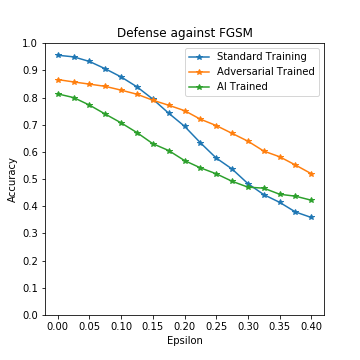
\includegraphics[scale=0.5]{Advsarial_code/figures/doc_defense_against_FGSM.png}\\
	Figure $n$: FGSM attack - Size of perturbation against accuracy of models. 
\end{center}

Although initially the Vanilla model out performs the other two models, given large enough perturbation the other models are more stable against FGSM attack.\\ 

When being perturbed by a universal adversarial attack the vanilla model always out preformed the models trained with defences against this exact attack. 

\begin{center}
	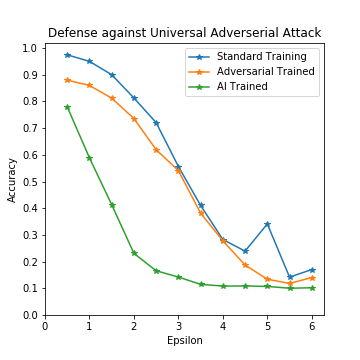
\includegraphics[scale=0.5]{Advsarial_code/figures/doc_defense_against_UAA.png}\\
	Figure $n + 1$: Universal adversarial attack - Size of perturbation against accuracy of models.
\end{center}

However, this could easily be caused by the wrong choice of variables, architecture, or that the models without defence converges quicker than those with defences.

%\subsubsection{Further Ideas}

%An idea we did not have time to implement was to use genetic algorithms to test different defence an attacking algorithms. The idea would be to pair image classifiers with a perturbation generators and then see how the pairs fair against one another, equip a score then breed these alogorithms. 
